\documentclass[8pt]{beamer}
\usetheme{Montpellier} 
\usepackage{lmodern}
\usepackage{amsmath}
\usepackage[utf8]{inputenc}
\usepackage[T1]{fontenc}
\usepackage{polski}
\usepackage[polish]{babel}


\newcommand{\argmax}[1]{\underset{#1}{\operatorname{arg}\,\operatorname{max}}\;}
\beamertemplatenavigationsymbolsempty

\makeatletter
\setbeamertemplate{footline}
{
  \leavevmode%
  \hbox{%
  \begin{beamercolorbox}[wd=.333333\paperwidth,ht=2.25ex,dp=1ex,center]{author in head/foot}%
    \usebeamerfont{author in head/foot}\insertshortauthor~~\beamer@ifempty{\insertshortinstitute}{}{(\insertshortinstitute)}
  \end{beamercolorbox}%
  \begin{beamercolorbox}[wd=.333333\paperwidth,ht=2.25ex,dp=1ex,center]{title in head/foot}%
    \usebeamerfont{title in head/foot}\insertshorttitle
  \end{beamercolorbox}%
  \begin{beamercolorbox}[wd=.333333\paperwidth,ht=2.25ex,dp=1ex,right]{date in head/foot}%
    \usebeamerfont{date in head/foot}\insertshortdate{}\hspace*{2em}
    \insertframenumber\hspace*{2ex} 
  \end{beamercolorbox}}%
  \vskip0pt%
}
\makeatother


\author[Adam Kosiorek]{Adam Kosiorek\\ \footnotesize pod kierunkiem prof. dr hab. B. Siemiątkowskiej}
\begin{document}
\title[Rozpoznawanie obiektów 3D na podstawie danych RGBD]{\HUGE Politechnika Warszawska\\ Wydział Mechatroniki \\ \ \\ \Large Rozpoznawanie obiektów 3D na podstawie danych RGBD} 
\date{11 lutego 2014} 

\thispagestyle{empty}
\titlepage
\thispagestyle{empty}
\frame{\frametitle{Spis treści}\tableofcontents}
\begin{document}

\section{Założenia i zakres pracy} 

\begin{frame}
  \setcounter{framenumber}{1}
  \frametitle{Założenia}
   
   Założeniem pracy jest zbadanie zagadnienia klasyfikacji obiektów 3D na podstawie zdjęć RGBD. Zdjęcia powinny byc zrobione kamerą Microsoft Kinect oraz być reprezentowane w formie chmur punktów. Ponadto zakłada się: \ \\
  \begin{itemize}
   \item Zaprojektowanie algorytmu rozpoznawania obrazów podejściem Bag of Words
   \item 
  \end{itemize}

\end{frame}

\begin{frame}{Zakres pracy}
\end{frame}


\section{Podejście Bag of Words}
\begin{frame}
  \frametitle{Bag of Words - Wprowadzenie}
  \begin{figure}
    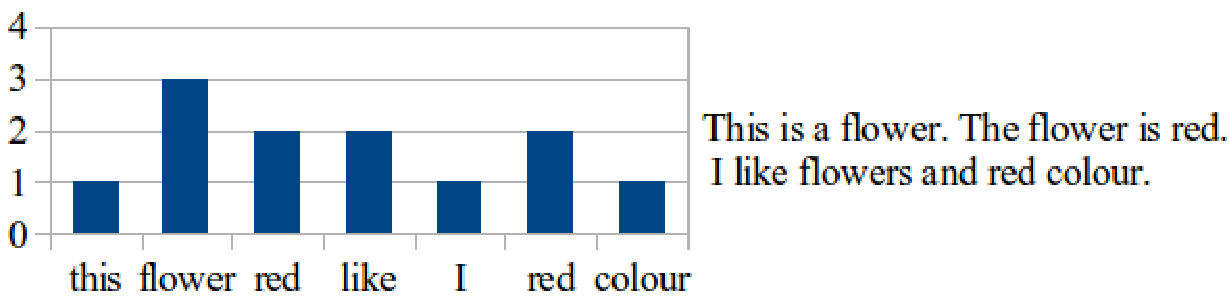
\includegraphics[scale=0.3]{../figs/bow_example-eps-converted-to}
  \end{figure}
  
  \begin{itemize}
   \item Częstośc występowania słów
   \item Usunięcie gramatyki, kolejności słów
   \item Histogram jako forma pośrednia
   \item Wymaga utworzenia słownika
   \item Reprezentacja rzadka w przypadku dużego słownika
   \item Używany m. in. do znajdowania rozkładu tematów w obrazie
  \end{itemize}


\end{frame}

\begin{frame}
	\frametitle{Bag of Words w obrazach}
	
	\begin{columns}
	
	 \begin{column}{6cm}
	 \begin{figure}
	   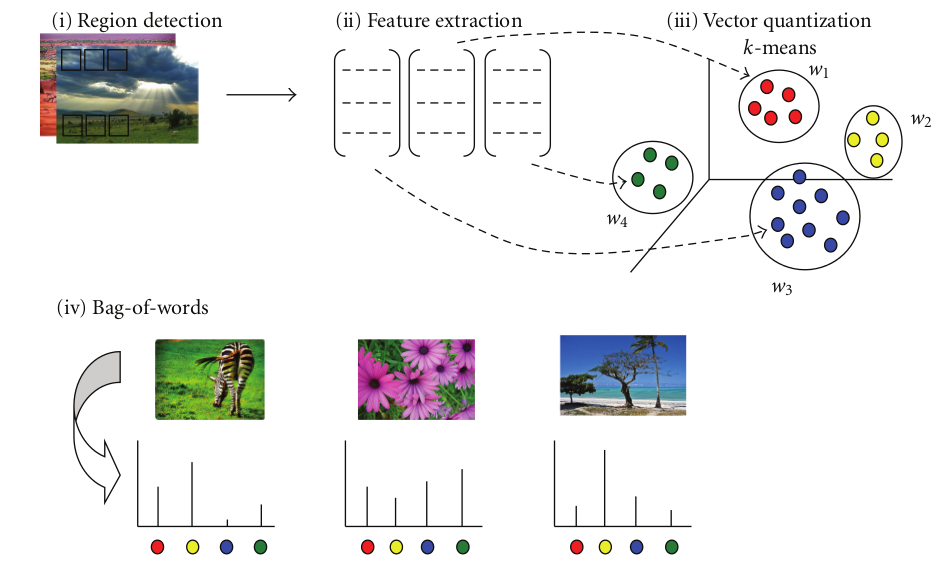
\includegraphics[scale=0.15]{../figs/tsai2012}
	   \end{figure}
	 \end{column}
	 
	 \begin{column}{3cm}
	  \footnotesize Grafika pochodzi z C. Tsai. \textit{Bag-of-words representation in image annotation: A review. ISN Artificial Intelligence, 2012}.
	 \end{column}

	\end{columns}

	\begin{enumerate}
	 \item Wykrycie punktów charakterystycznych
	 \begin{itemize}
	  \item współrzędne (x, y) oraz skala obrazka
	 \end{itemize}

	 \item Opisanie otoczenia wykrytych punktów
	 \begin{itemize}
	  \item opis jednoznaczny, zazwyczaj poprzez histogram gradientów
	 \end{itemize}
	 \item Budowanie słownika i kwantyzacja
	 \begin{itemize}
	  \item punkty układają się w obszary, które można wykryć - klasteryzacja
	 \end{itemize}
	 \item Klasyfikacja
	 \begin{itemize}
	  \item klasyfikator uczący się - Support Vector Machine, Modele graficzne, Boosting
	 \end{itemize}
	\end{enumerate}


	
\end{frame}


\begin{frame}
	\frametitle{}
\end{frame}

\begin{frame}
	\frametitle{}
\end{frame}

\begin{frame}
	\frametitle{}
\end{frame}

\begin{frame}
	\frametitle{}
\end{frame}

\begin{frame}
	\frametitle{}
\end{frame}

\end{document}

